\documentclass[12pt,a4paper,oneside]{book} 

%%%%%%%%%%%%%%%%%%%%%%%%%%%%%%%%%%%%%%%%%%%%%%%%%%%%%%%%%%%%%%%%%%%%%%%%

\usepackage{ifthen}
\usepackage{graphicx}
\usepackage[dvips]{epsfig}
\usepackage{enumerate}
\usepackage{calc}
\usepackage{multicol} 
\usepackage{titlesec}
%\usepackage{showkeys}

%%%%%%%%%%%%%%%%%%%%%%%%%%%%%%%%%%%%%%%%%%%%%%%%%%%%%%%%%%%%%%%%%%%%%%%%

\usepackage{a4}
\usepackage{amsfonts}
\usepackage{amssymb}
\usepackage{epsfig}

%%%%%%%%%%%%%%%%%%%%%%%%%%%%%%%%%%%%%%%%%%%%%%%%%%%%%%%%%%%%%%%%%%%%%%%%

\usepackage{t1enc,times}
\usepackage{latexsym,amssymb}
\usepackage{amsmath}
\usepackage{amstext}
%\usepackage[T1]{fontenc}
%\usepackage{cmbright}
\usepackage{pifont}
\usepackage{marvosym}
%\usepackage{pslatex}
% \usepackage{stmaryrd} %=== > dont have it installed on system, doesnt look like it's a compulsory package anyway
%\usepackage{txfonts}  

%%%%%%%%%%%%%%%%%%%%%%%%%%%%%%%%%%%%%%%%%%%%%%%%%%%%%%%%%%%%%%%%%%%%%%%%%%%%%%%

\usepackage[titletoc]{appendix}
\usepackage{mathrsfs}

%%%%%%%%%%%%%%%%%%%%%%%%%%%%%%%%%%%%%%%%%%%%%%%%%%%%%%%%%%%%%%%%%%%%%%%%%%%%%%%

\usepackage{fancybox} 
\usepackage{fancyhdr}
\usepackage{fullpage}

%%%%%%%%%%%%%%%%%%%%%%%%%%%%%%%%%%%%%%%%%%%%%%%%%%%%%%%%%%%%%%%%%%%%%%%%%%%%%%%

%\usepackage{url}    
%\ExecuteOptions{dvips}
%\usepackage[pdftex,colorlinks=true]{hyperref}
%\hypersetup{backref,pdfpagemode=UseThumbs,pdfstartview=Fit,
%pdfpagelayout=SinglePage,pdfstartpage=1,colorlinks=true,menucolor=msc,
%anchorcolor=msc,pagecolor=msc,urlcolor=rfr,breaklinks=true,hyperfootnotes=true}

%%%%%%%%%%%%%%%%%%%%%%%%%%%%%%%%%%%%%%%%%%%%%%%%%%%%%%%%%%%%%%%%%%%%%%%%%%%%%%%

\pagestyle{fancy}
\fancyhf{} 
%\renewcommand{\headrulewidth}{1pt}
%\renewcommand{\footrulewidth}{1pt}
\renewcommand{\headwidth}{\textwidth}
\fancyhead[LE]{\leftmark}
\fancyhead[RO]{\small \rightmark}
\fancyfoot[C]{\thepage}

%%%%%%%%%%%%%%%%%%%%%%%%%%%%%%%%%%%%%%%%%%%%%%%%%%%%%%%%%%%%%%%%%%%%%%%%%%%%%%%

\tolerance 4000
\textwidth 17.00cm
\topmargin -0.30cm
\oddsidemargin -0.25cm
\evensidemargin -0.25cm
\textheight 23.00cm
%\headsep 12pt
\headheight 15pt
\footskip 60pt
%\parindent 12pt

%%%%%%%%%%%%%%%%%%%%%%%%%%%%%%%%%%%%%%%%%%%%%%%%%%%%%%%%%%%%%%%%%%%%%%%%%%%%%%%

\renewcommand{\rmdefault}{ptm}  % times
\renewcommand{\rmdefault}{phv}  % helvetica
\renewcommand{\rmdefault}{pbk}  % bookman
\renewcommand{\rmdefault}{ppl}  % palatino
\renewcommand{\sfdefault}{phv}  % helvetica as sans serif
\renewcommand{\ttdefault}{pcr}  % courier as fixed width
\renewcommand{\tabcolsep}{8pt}
\renewcommand{\arraystretch}{1.25}

%%%%%%%%%%%%%%%%%%%%%%%%%%%%%%%%%%%%%%%%%%%%%%%%%%%%%%%%%%%%%%%%%%%%%%%%%%%%%%%

\newcommand{\Lim}[1]{\raisebox{0.5ex}{\scalebox{0.8}{$\displaystyle \lim_{#1}\;$}}}

%%%%%%%%%%%%%%%%%%%%%%%%%%%%%%%%%%%%%%%%%%%%%%%%%%%%%%%%%%%%%%%%%%%%%%%%%%%%%%%

\def\nn{\nonumber}
\def\f{{\frac}}
\def\pa{{\partial}}
\def\d{{\rm d}}
\def\l{\left}
\def\r{\right}
\def\Mpl{M_{_{\rm Pl}}}

%%%%%%%%%%%%%%%%%%%%%%%%%%%%%%%%%%%%%%%%%%%%%%%%%%%%%%%%%%%%%%%%%%%%%%%%%%%%%%%

\def\done{\marginpar {\scriptsize DONE}}
\def\check{\marginpar {\scriptsize CHECK}}

%%%%%%%%%%%%%%%%%%%%%%%%%%%%%%%%%%%%%%%%%%%%%%%%%%%%%%%%%%%%%%%%%%%%%%%%%%%%%%%

\begin{document}

%%%%%%%%%%%%%%%%%%%%%%%%%%%%%%%%%%%%%%%%%%%%%%%%%%%%%%%%%%%%%%%%%%%%%%%%%%%%%%%

\baselineskip 20pt

%%%%%%%%%%%%%%%%%%%%%%%%%%%%%%%%%%%%%%%%%%%%%%%%%%%%%%%%%%%%%%%%%%%%%%%%%%%%%%%

\pagenumbering{roman}

%%%%%%%%%%%%%%%%%%%%%%%%%%%%%%%%%%%%%%%%%%%%%%%%%%%%%%%%%%%%%%%%%%%%%%%%%%%%%%%

\thispagestyle{empty}
\topskip 15pt
\hrule\hrule\hrule\hrule\hrule
\vskip 20pt
\centerline{\Huge \bf Generation of gravitational waves} 
\vskip 15pt
\centerline{\Huge \bf during inflation} 
\vskip 20pt
\hrule\hrule\hrule\hrule\hrule
\vskip 30pt
\centerline{\Large A mini-project report}
\vskip 8pt
\centerline{\Large submitted in partial fulfilment 
for the award of the degree of}
\vskip 8pt
\centerline{\Large B.S \& M.S in Physics}
%\vskip 8pt
%\centerline{\Large in}
%\vskip 8pt 
%\centerline{\Large Physics}
\vskip 8pt
\centerline{\Large by}
\vskip 8pt
\centerline{\Large \bf Poruri Sai Rahul}
\vskip 8pt
\centerline{\Large under the guidance of}
\vskip 8pt
\centerline{\Large  Dr.~L.~Sriramkumar}
\vskip 30pt 
\begin{center}

\epsfig{file=iitm.eps, width=3.0cm, height=3.0cm} % needed to convert .ps ext to .eps ext.
\end{center}
\vskip 8pt 
\centerline{\Large \bf Department of Physics}
\vskip 8pt 
\centerline{\Large \bf Indian Institute of Technology Madras}
\vskip 8pt 
\centerline{\Large \bf Chennai~600036, India}
\vskip 8pt
\centerline{\Large \bf June~2015}
%%%%%%%%%%%%%%%%%%%%%%%%%%%%%%%%%%%%%%%%%%%%%%%%%%%%%%%%%%%%%%%%%%%%%%%%%%%%%%%

\newpage\topskip 40pt
\centerline{\Large CERTIFICATE}
\thispagestyle{empty}
\vskip 20pt\noindent 
This is to certify that the project titled {\bf Generation of Gravitational
waves during Inflation} is a bona fide record of work done by 
{\bf Poruri Sai Rahul} towards the partial fulfilment of the 
requirements of the B.S \& M.S degree in Physics at the Indian 
Institute of Technology, Madras, Chennai 600036, India.
\vskip 120pt
\hspace{240pt}(L.~Sriramkumar, Project supervisor)

%%%%%%%%%%%%%%%%%%%%%%%%%%%%%%%%%%%%%%%%%%%%%%%%%%%%%%%%%%%%%%%%%%%%%%%%%%%%%%%

\newpage\topskip 40pt
\thispagestyle{empty}
\centerline{\Large ACKNOWLEDGEMENTS}
\vskip 20pt\noindent 

I cannot express in words my gratitude to {\bf Dr. L.~Sriramkumar} 
for guiding me, regarding my work and my personal life. I would also
like to thank V.~Sreenath and Debika Choudhury for helping me 
with my project and for clarifying my doubts.

I would also like to thank my family and my friends, especially Shashi Kunwar
and Preeti Saryan, who have kept me on my toes over the last few years.
 
 %%%%%%%%%%%%%%%%%%%%%%%%%%%%%%%%%%%%%%%%%%%%%%%%%%%%%%%%%%%%%%%%%%%%%%%%%%%%%%%

\newpage\topskip 40pt
\thispagestyle{empty}
\centerline{\Large ABSTRACT}
\vskip 20pt\noindent 

The precision with which inhomogeneities in the Cosmic Microwave Background, CMB for short, are being measured
has increased tremendously over the years, thanks to the efforts of the Planck and the WMAP missions. 
We are currently in an era of precision cosmology. The theory of inflation predicts the presence of such 
inhomogeneities. In this work, I studied the theory behind the generation and evolution of tensor perturbations, 
otherwise referred to as primordial gravitational waves. I also numerically estimate the power spectrum of such 
perturbations for two different models of inflation.
%%%%%%%%%%%%%%%%%%%%%%%%%%%%%%%%%%%%%%%%%%%%%%%%%%%%%%%%%%%%%%%%%%%%%%%%%%%%%%%

\newpage
\thispagestyle{empty}
\tableofcontents
\newpage

%%%%%%%%%%%%%%%%%%%%%%%%%%%%%%%%%%%%%%%%%%%%%%%%%%%%%%%%%%%%%%%%%%%%%%%%%%%%%%%

\newpage
\thispagestyle{empty}
\listoffigures
\newpage

%%%%%%%%%%%%%%%%%%%%%%%%%%%%%%%%%%%%%%%%%%%%%%%%%%%%%%%%%%%%%%%%%%%%%%%%%%%%%%%

\pagenumbering{arabic}

%%%%%%%%%%%%%%%%%%%%%%%%%%%%%%%%%%%%%%%%%%%%%%%%%%%%%%%%%%%%%%%%%%%%%%%%%%%%%%%

\chapter{Introduction}

\paragraph*{} Inflation refers to a period of rapid expansion during the early stages of the radiation dominated epoch of our universe. 
Inflation solved two of the biggest drawbacks of the Hot Big Bang model i.e the horizon problem and the flatness problem. For an in-depth 
review of the horizon problem and how one can overcome it using inflation, refer to %~\cite{Sriramkumar L - 2009}
. The amount of inflation 
needed to solve the horizon problem can be estimated by looking at the ratio of the backward and forward light cones at the epoch of 
decoupling. It is expressed in terms of number of e-folds defined as

\begin{equation}
N = \int^t_{t_i} {\rm d}t H = {\rm ln}\left(\frac{a(t)}{a_0}\right)
\end{equation}

\noindent where $a(t)$ is the scale factor of the universe. Upon substituting the necessary values for $a(t)$, one can see that approximately 60 e-folds of inflation are needed to 
overcome the horizon problem.

\section{Conventions and notations}

\paragraph*{} Before we go any further, I shall list the convention and notation adopted in this work. I work in $(3+1)-$ dimentions, unless 
mentioned otherwise and I adopt the metric signature $(+,-,-,-)$. Greek indices denote all spacetime coordinates where as Latin indices 
refer to spatial coordinates specifically. I define the Planck mass $M_P=\left(8\pi G\right)^{-1/2}$. Cosmic time is denoted using $t$ and 
an overdot denotes differentiation with respect to cosmic time where as the conformal time is denoted using $\eta$ and an overprime 
denotes differentiation with respect to conformal time.

\section{Driving inflation}

In order to achieve inflation, it is necessary that

\begin{equation}\label{eq:1}
\ddot{a} > 0
\end{equation}

\paragraph*{} In a spatially flat, smooth, Friedmann universe, the line element is described by

\begin{equation}
{\rm d}s^2 = {\rm d}t^2 - a^2(t){\rm d}{\bf x}^2 = a^2(\eta)\left({\rm d}\eta^2 - {\rm d}{\bf x}^2\right)
\end{equation}

\noindent and for such a line element, the Einstein's equations can be rewritten as the following two Friedmann equations

\begin{equation}\label{eq:F1}
\left(\frac{\dot{a}}{a}\right)^2 = H^2 = \left(\frac{8\pi G}{3}\right)\rho
\end{equation}

\begin{equation}\label{eq:F2}
\left(\frac{\ddot{a}}{a}\right) = \dot{H} + H^2= -\left(\frac{4\pi G}{3}\right)(\rho + 3p)
\end{equation}

\noindent where $\rho$ and ${\rm p}$ denote the energy density and pressure of the field driving the expansion.

\paragraph*{} From ~\ref{eq:1} and ~\ref{eq:F2}, it is straight forward to see that

\begin{equation}
(\rho + 3p) < 0
\end{equation}

\noindent is a necessary condition for the field that drives inflation. One can check that neither matter, for which ${\rm p} = \rho/3$, 
nor radiation, for which ${\rm p} = 0$, satisfies the necessary condition. We can therefore assume that, under the necessary conditions, 
a generic scalar field $\phi$ and a corresponding potential $V(\phi)$ govern the inflationary paradigm. A scalar field that drives inflation 
is also referred to as an Inflaton.

\paragraph*{} One can write the corresponding action and the stress-energy tensor for such a scalar field as

\begin{equation}\label{eq:act}
S(\phi) = \int {\rm d}^4x \sqrt{-g}\left[ \left(\frac{1}{2}\right)\left(\partial^{\lambda}\phi \partial_{\lambda}\phi\right) - V(\phi)\right]
\end{equation}

\begin{equation}\label{eq:se}
T^{\mu}_{\nu} = \partial^{\mu}\phi \partial_{\nu}\phi -\delta^{\mu}_{\nu}\left[\left(\frac{1}{2}\right)\left(\partial^{\lambda}\phi \partial_{\lambda}\phi\right) - V(\phi)\right]
\end{equation}

\noindent We can also derive the equations of motion for the scalar field from ~\ref{eq:act} to be

\begin{equation}
\ddot{\phi} + 3H\dot{\phi} + V_{\phi} = 0
\end{equation}

\noindent where $V_{\phi} = \left({\rm d}V/{\rm d}\phi\right)$

\section{Metric perturbations}

\paragraph*{} Inhomogeneities in the CMB are one part in $10^5$ and it can be inferred that they should be much smaller at earlier 
epochs given the expanding nature of our universe. We can therefore study the generation and evolution of such perturbations using 
linear perturbation theory. While higher-order perturbations have been discovered in recent CMB observations, they are beyond the 
scope of this work. The linear perturbations in Friedmann metric can be classified as scalar, vector and tensor perturbations. 
For the scope of this work, I restrict myself to tensor perturbations of the metric, which can be represented as

\begin{equation}
{\rm d}s^2 = {\rm d}t^2 - a^2(t)(\delta_{ij} + h_{ij}){\rm d}x^i{\rm d}x^j
\end{equation}

\noindent Tensor perturbations are also referred to as gravitational waves, characterized by a transverse, traceless matrix $h_{ij}$. 
The perturbed Einstein equations corresponding to the above metric with tensor perturbations are

\begin{equation}
\delta G^0_0 = \delta G^0_i = 0
\end{equation}

\begin{equation}
\delta G^i_j = -\left(\frac{1}{2}\right)\left(\ddot{h}_{ij} + 3H\dot{h}_{ij} - \frac{1}{a^2}\nabla ^2h_{ij}\right)
\end{equation}

\paragraph*{} Similarly, one can write the perturbed stress-energy tensor as

\begin{equation}
\delta T^0_0 = \delta\rho, \delta T^0_i = \left(\nabla_i\delta\sigma\right)  {\rm and}  \delta T^i_j = -\delta p\delta^i_j
\end{equation}

\noindent In the absence of anisotropic stresses i.e if $\delta T^i_j = 0$, we get that

\begin{equation}\label{tp}
\ddot{h} + 3H\dot{h} - \left(\frac{1}{a^2}\right)\nabla ^2h = 0
\end{equation}

\section{Quantization of perturbations}

\paragraph*{} Upon quantization, we can write the tensor perturbations $\hat{h}$ in terms of it's Fourier modes $h_k$ as

\begin{equation}
\hat{h}(\eta, {\bf x}) = \int \frac{{\rm d}^3\bf{k}}{(2\pi)^{3/2}} \left[\hat{a_k}h_k(\eta)e^{i\bf{k\cdot x}}+ \hat{a_k}^{\dagger}h_k^{*}(\eta)e^{-i\bf{k\cdot x}}\right] 
\end{equation}

\noindent where the creation and annihilation operators, $\hat{a_k}$ and $\hat{a_k}^{\dagger}$, follow the standard commutation relations. At the linear order in perturbations that we are working in, the power spectrum of the tensor perturbations can be characterized by the two point function of the quantum field $\hat{h}$. The power spectrum of the tensor perturbations ${\mathcal{P}}_T(k)$ and the two point function are related by

\begin{equation}
\int^{\infty}_0 {\mathcal{P}}_T(k) = \int d^3{\bf{k}}\int\frac{d^3(\bf{x}-\bf{x'})}{(2\pi)^3}\langle 0|P(\eta,{\bf{x}})P(\eta, {\bf{x'}})|\rangle \times e^{-i{\bf{\left[k \cdot (x-x')\right]}}}
\end{equation}

\noindent where $|0\rangle$ is the vacuum state defined as $\hat{a_k}|0\rangle = 0 \forall {\bf{k}}$. Using the earlier relation, one can obtain the power spectrum as

\begin{equation}\label{eq:tps}
{\mathcal{P}}_T(k) = 2 \left(\frac{k^3}{2\pi^2}\right) |h_k|^2
\end{equation}

\noindent where the factor of 2 is needed to take into account the two states of polarization, $+$ and $\times$, of the gravitational waves.

%%%%%%%%%%%%%%%%%%%%%%%%%%%%%%%%%%%%%%%%%%%%%%%%%%%%%%%%%%%%%%%%%%%%%%%%%%%%%%%

\chapter{Inflationary models}

%%%%%%%%%%%%%%%%%%%%%%%%%%%%%%%%%%%%%%%%%%%%%%%%%%%%%%%%%%%%%%%%%%%%%%%%%%%%%%%

\paragraph*{} From \ref{eq:se}, one can write the individual components of the stress-energy tensor for a scalar field $\phi$ as

\begin{equation}\label{eq:se1}
T^{0}_{0} = \left[\left(\frac{\dot{\phi}^2}{2}\right) +V(\phi)\right] = \rho 
\end{equation}

\begin{equation}\label{eq:se2}
T^{i}_{j} = -\left[\left(\frac{\dot{\phi}^2}{2}\right) - V(\phi)\right]\delta^{i}_{j} = -p\delta^i_j
\end{equation}

\paragraph*{} Using \ref{eq:se1} and \ref{eq:se2}, one can rewrite \ref{eq:F1} and \ref{eq:F2} as

\begin{equation}
 \dot{H} = \frac{-\dot{\phi}^2}{2M_P^2}
\end{equation}

\begin{equation}
H^2 = \left(\frac{1}{3M_P^2}\right)\left[\frac{\dot{\phi}^2}{2} + V_{\phi}\right]
\end{equation}

\noindent One can now express the scalar field $\phi$ and the potential $V$ in terms of cosmic time ${\rm t}$ as

\begin{equation}
\phi(t)= \sqrt{2}M_P \int dt \sqrt{-\dot{H}}
\end{equation}

\begin{equation}
V(t) = M_P^2\left(3H^2 + \dot{H}\right)
\end{equation}

\section{Power law inflation}

\paragraph*{} Assuming that the scale factor has a power-law form during inflation i.e

\begin{equation}\label{eq:power}
a(t) = a_0t^q
\end{equation}

\noindent one can see that the scalar field and the potential that drive the inflation have the form

\begin{equation}
\frac{\phi(t)}{M_P} =\sqrt{\left(2q\right)} {\rm ln}\left[\sqrt{\left(\frac{V_0}{(3q-1)q}\right)}\left(\frac{t}{M_P}\right)\right]
\end{equation}

\begin{equation}
V(\phi) = V_0\exp\left[-\sqrt{\frac{2}{q}}\left(\frac{\phi}{M_P}\right)\right]
\end{equation}

\paragraph*{} In terms of e-fold ${\rm N}$, we can rewrite $\phi(t)$ as

\begin{equation}
\phi(N) = \sqrt{\left(\frac{2}{q}\right)} N - \sqrt{\left(2q\right)}{\rm ln}t_0
\end{equation}

\paragraph*{} Similarly, one can rewrite the Hubble parameter $H$ in terms of e-fold time as 

\begin{equation}
H(N) = H_0\exp^{-N/q}
\end{equation}

\noindent We also introduce a new parameter $\epsilon_1(N)$, which is defined as

\begin{equation}
\epsilon_1(N) = \phi'(N) = \sqrt{\left(\frac{2}{q}\right)}
\end{equation}

Further, by substituting $h = \left(u/a\right)$, we can rewrite \ref{tp} as

\begin{equation}\label{eq:MS}
u''_k + \left[k^2 - \left(\frac{a''}{a}\right)\right]u_k = 0
\end{equation}

\noindent and the power spectrum governing \ref{eq:tps}
\begin{equation}
{\mathcal{P}}_T(k) = 2 \left(\frac{k^3}{2\pi^2}\right) |h_k|^2 = 2 \left(\frac{k^3}{2\pi^2}\right) \left(\frac{|u_k|}{a}\right)^2
\end{equation}

\subsection{The Bunch-Davies initial conditions}

\begin{equation}\label{eq:bd}
\Lim{\left(k/aH\right) \rightarrow \infty} u_k(\eta) \rightarrow \left(\frac{1}{\sqrt{2k}}\right){\rm e}^{-ik\eta}
\end{equation}

\subsection{Tensor power spectrum}

\paragraph*{} Using the scale factor \ref{eq:power}, one can obtain that

\begin{equation}
u_k(\eta) = \left(\frac{-\pi\eta}{4}\right)^{1/2}{\rm e}^{i[\nu+(1/2)](\pi/2)}{\rm H}_{\nu}^{(1)}(-k\eta)
\end{equation}

\noindent is a solution to \ref{eq:MS} which satisfies the initial conditions \ref{eq:bd}, where $\nu = [\gamma + (1/2)]$ and 
${\rm H}_{\nu}^{(1)}$ is the Hankel funciton of the first kind and of order $\nu$.

\paragraph*{} In the super-Hubble limit $($ i.e as $(-k\eta \rightarrow 0))$, one can approximate the Hankel function to

\noindent It is straight forward to see that the tensor amplitude $h_k$ reaches a constant value and that the tensor power spectrum
evaluated at super-Hubble scales can be written as

\begin{equation}
\mathcal{P}_T(k) = A_T\bar{\mathcal{H}}^2\left(\frac{k}{\mathcal{\bar{H}}}\right)^{2(\gamma+2)}
\end{equation}

\noindent where

\begin{equation}
A_T = \left[\frac{1}{\pi^3M_P^2}\right]\left(\frac{|\Gamma(\nu)|^2}{2^{(2\gamma+1)}}\right)
\end{equation}

\section{Small field inflation}

\begin{equation}
V = V_0\left[1 - \left(\frac{\phi}{\mu}\right)^p\right]
\end{equation}

%%%%%%%%%%%%%%%%%%%%%%%%%%%%%%%%%%%%%%%%%%%%%%%%%%%%%%%%%%%%%%%%%%%%%%%%%%%%%%%

\chapter{Numerical results}

\paragraph{} In this section, I describe the procedure adopted to numerically evaluate the tensor power spectrum of gravitational waves in a power-law inflationary scenario. Recall that conventionally, e-fold $N$ is defined as $N = {\rm ln}(a/a_0)$, where $N$ gives an estimate of the amount of inflation needed to solve the horizon problem. Also, note that an overdot represents differentiation with respect to coordinate time $t$ and that an overprime represents differentiation with respect to conformal time $\eta$.

\section{Power-law inflation}

\paragraph{} Assuming an inflationary potential $V(\phi)$ of the form

\begin{equation}
V(\phi) = V_0 \exp\left[-\sqrt{\frac{2}{q}}\left(\phi - \phi_0\right)\right]
\end{equation}

\noindent where $\phi$ represents the scalar field driving inflation and $q$ is the power-law index.

\paragraph*{} Recall that the equation describing the evolution of the scalar field $\phi$ is

\begin{equation}
\ddot{\phi} + 3H\dot{\phi} + V_{\phi} = 0
\end{equation}

\noindent which can then be written in terms of e-fold time $N$ as

\begin{equation}
\frac{{\rm d}^2\phi}{{\rm d}N^2} + \left[3 - \frac{1}{2}\left(\frac{{\rm d}\phi}{{\rm d}N}\right)^2\right]\frac{{\rm d}\phi}{{\rm d}N} + \left[6 - \left(\frac{{\rm d}\phi}{{\rm d}N}\right)^2\right]\frac{1}{2V(\phi)}\frac{{\rm d}V(\phi)}{{\rm d}N} = 0
\end{equation}

\noindent Note that I've made used of the following definition for H to arrive at the above expression

\begin{equation}
H^2 = \frac{2V(\phi)}{3-(\frac{{\rm d}\phi}{{\rm d}N})^2}
\end{equation}

\paragraph*{} I numerically integrated the above second order differential equation from e-fold time $N = 0$ to $N = 70$ while assuming that $\phi_0 = 1$ and $\frac{{\rm d}\phi}{{\rm d}N}_0 = \frac{\sqrt{2q}}{t_0}\frac{1}{H_0}$ using a fourth-order Runge-Kutta method, implemented in Python.

\begin{figure}
\begin{center}
\includegraphics[scale=0.5]{phi_vs_N_power_law.png}
\caption[Plot of $\phi(N)$ vs $N$ during power law inflation]{Plot of $\phi(N)$ vs $N$ during power law inflation}
\end{center}
\end{figure}

\begin{figure}
\begin{center}
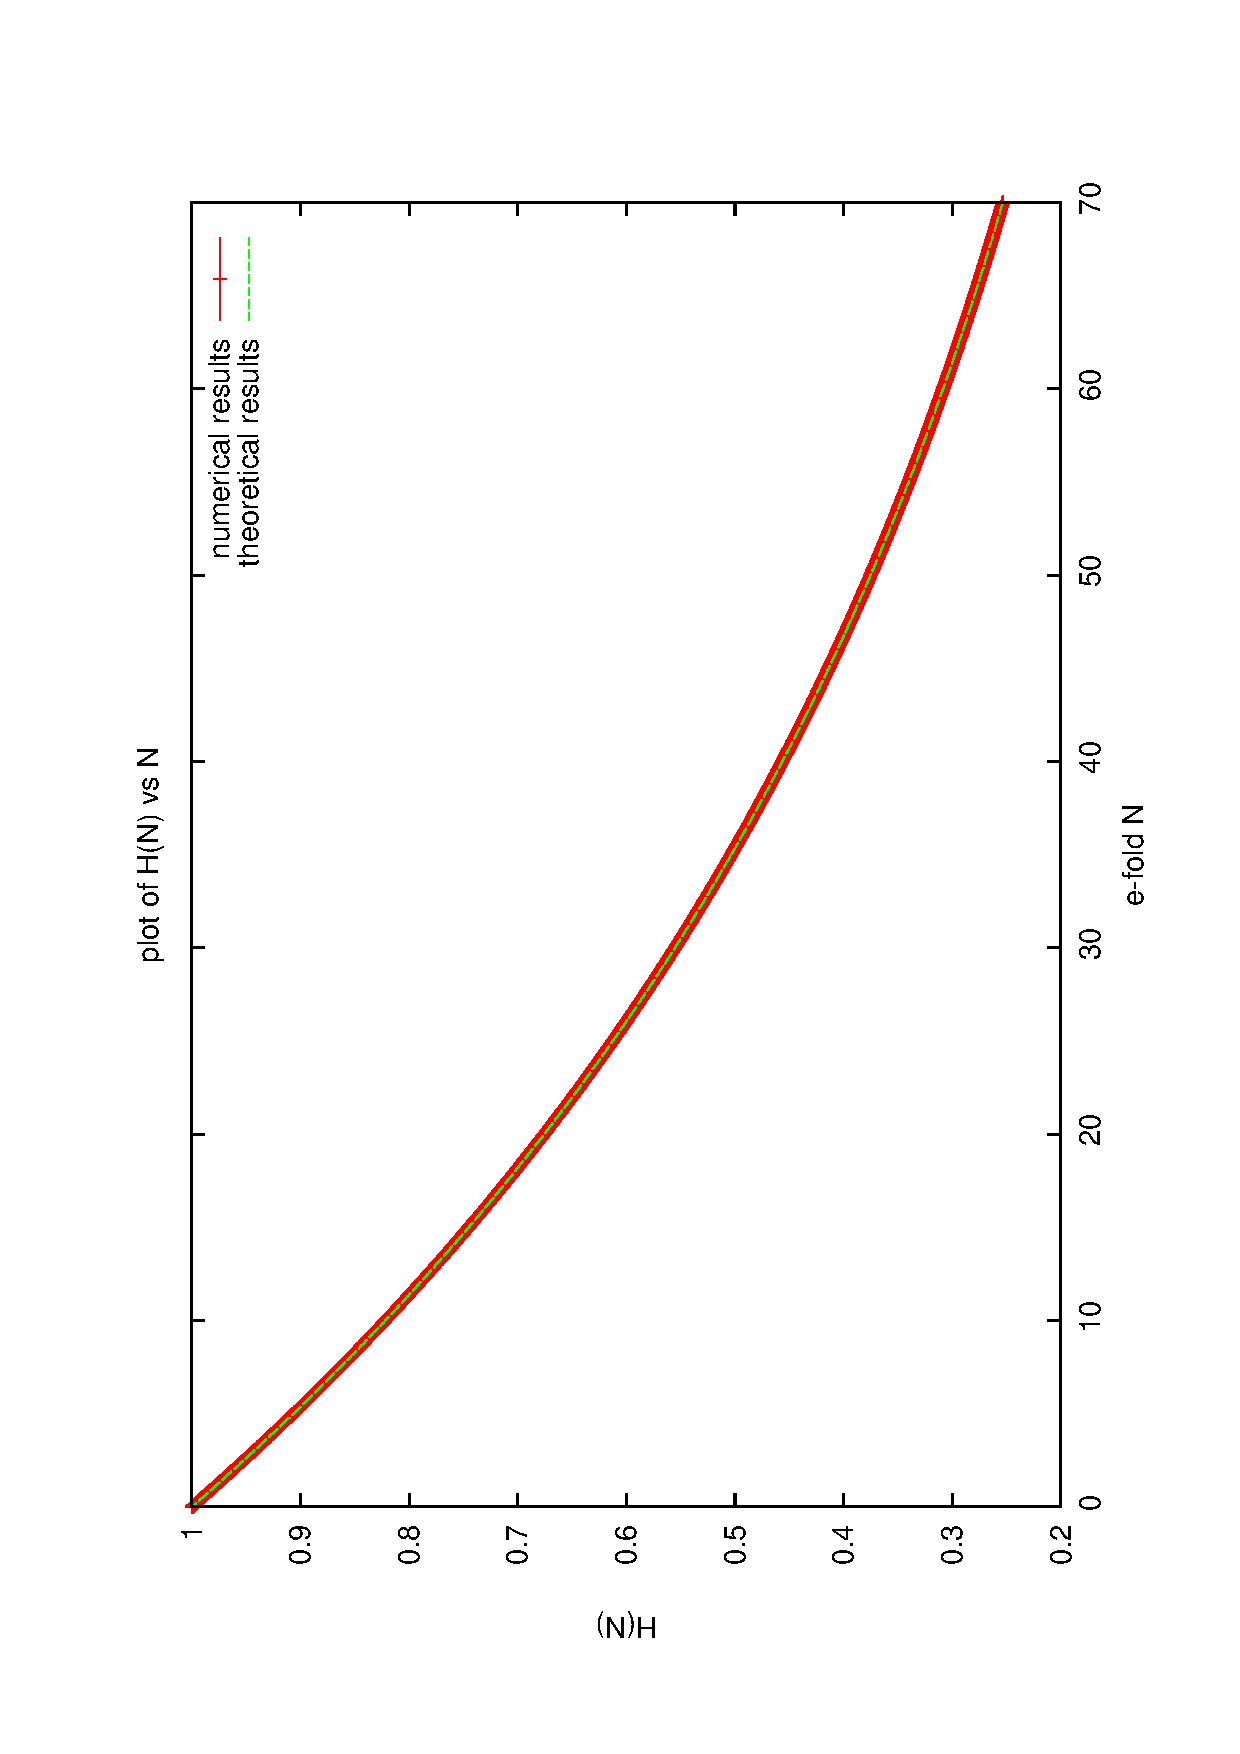
\includegraphics[scale=0.5]{H_vs_N_power_law.png}
\caption[Plot of $H(N)$ vs $N$ during power law inflation]{Plot of $H(N)$ vs $N$ during power law inflation}
\end{center}
\end{figure}

\begin{figure}
\begin{center}
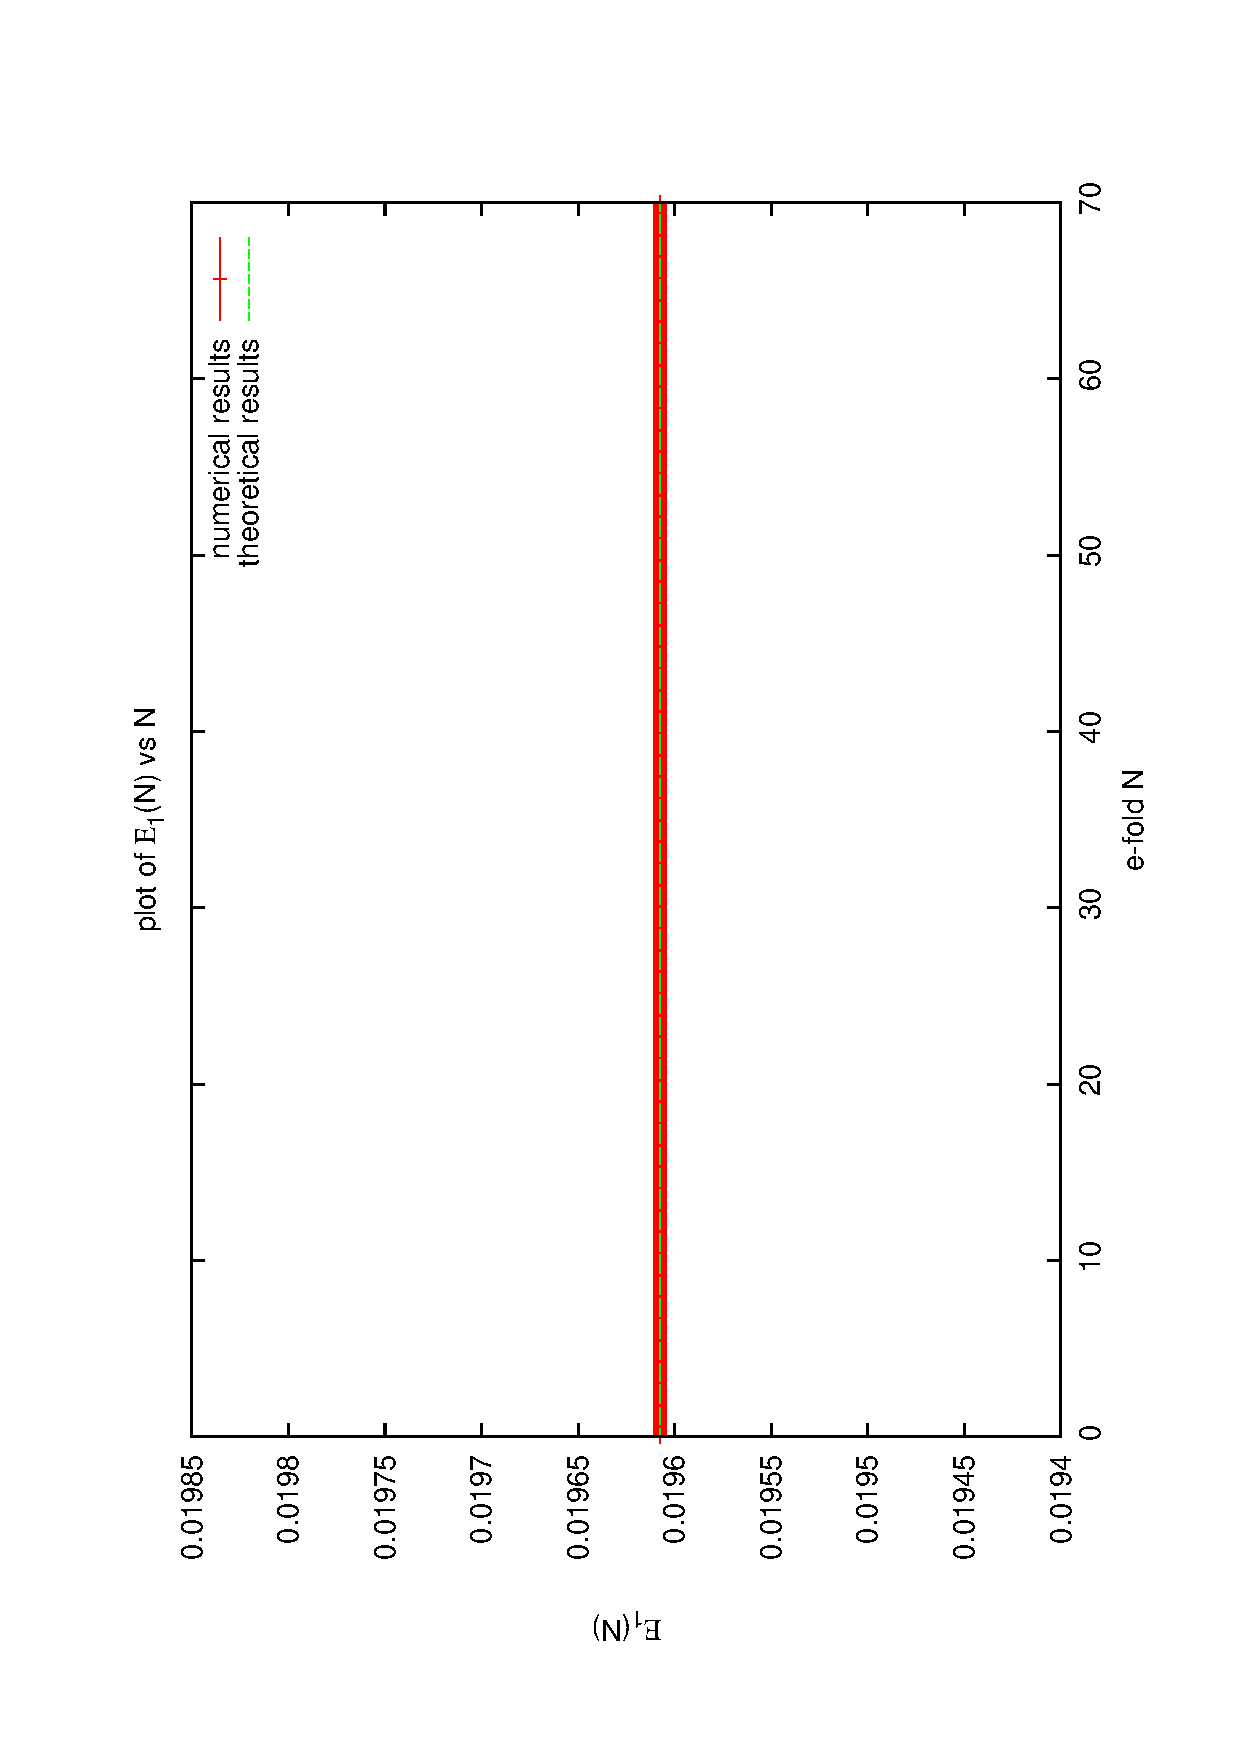
\includegraphics[scale=0.5]{eps1_vs_N_power_law.png}
\caption[Plot of $\epsilon 1(N)$ vs $N$ during power law inflation]{Plot of $\epsilon 1(N)$ vs $N$ during power law inflation}
\end{center}
\end{figure}

\paragraph*{} Recall that the equation governing the tensor perturbations in the metric is

\begin{equation}
\ddot{h} + 3H\dot{h} - \frac{1}{a^2}\nabla ^2h = 0
\end{equation}

\noindent which, in fourier space, becomes

\begin{equation}
\ddot{h}_k + 3H\dot{h}_k + \frac{k^2}{a^2}h_k = 0
\end{equation}

\paragraph*{} Rewriting the above equation in terms of e-fold time, we arrive at

\begin{equation}
\frac{{\rm d}^2h_k}{{\rm d}N^2} +\left (3+\frac{1}{H}\frac{{\rm d}H}{{\rm d}N}\right)\frac{{\rm d}h_k}{{\rm d}N} + \frac{k^2}{a^2H^2}h_k = 0
\end{equation}

\paragraph*{} The above equation was numerically integrated using a fourth order Runge-Kutta method, implemented in Python. It is to be noted that $h_k$ was evolved for various values of k, ranging from $10^{-6}$ to $10^{0}$. Corresponding initial and final limits on e-fold time N were placed by estimating the time when the modes are well inside the Hubble scale i.e $k/aH =  100$ and when the modes are well outside the Hubble scale i.e $k/aH =  10^{-5}$. The initial values for $h_k$ and $\frac{{\rm d}h_k}{{\rm d}N}$ were set to be

\begin{equation}
h_k  = \frac{1}{\sqrt{2k_0}a(N)}
\end{equation}

\begin{equation}
\frac{{\rm d}h_k}{{\rm d}N} = -\frac{1}{\sqrt{2k_0}a(N)} - \frac{i\sqrt{(k0/2)}}{a^2(N)H(N)}
\end{equation}

\paragraph*{} Having successfully obtained a numerical solution of $h_k$, we can evaluate the tensor power spectrum by using the formula %~\cite{Kodama:1985bj}

\begin{equation}
P_T(k) = 2 \left(\frac{k^3}{2\pi^2}\right) |h_k|^2
\end{equation}

\begin{figure}
\begin{center}
\includegraphics[scale=0.5]{power_spectrum_power_law.png}
\caption[Tensor power spectrum during power law inflation]{Tensor power spectrum during power law inflation}
\end{center}
\end{figure}

\section{Small field inflation}

\paragraph*{} Similarly, if one considers the potential function that drives inflation to be of the form

\begin{equation}
V(\phi) = V_0\left[1-\left(\frac{\phi}{\mu}\right)^p\right]
\end{equation}

\noindent commonly referred to as small field inflation, the scalar field, the Hubble parameter and $\epsilon$ can all be numerically estimated to be

\begin{figure}
\begin{center}
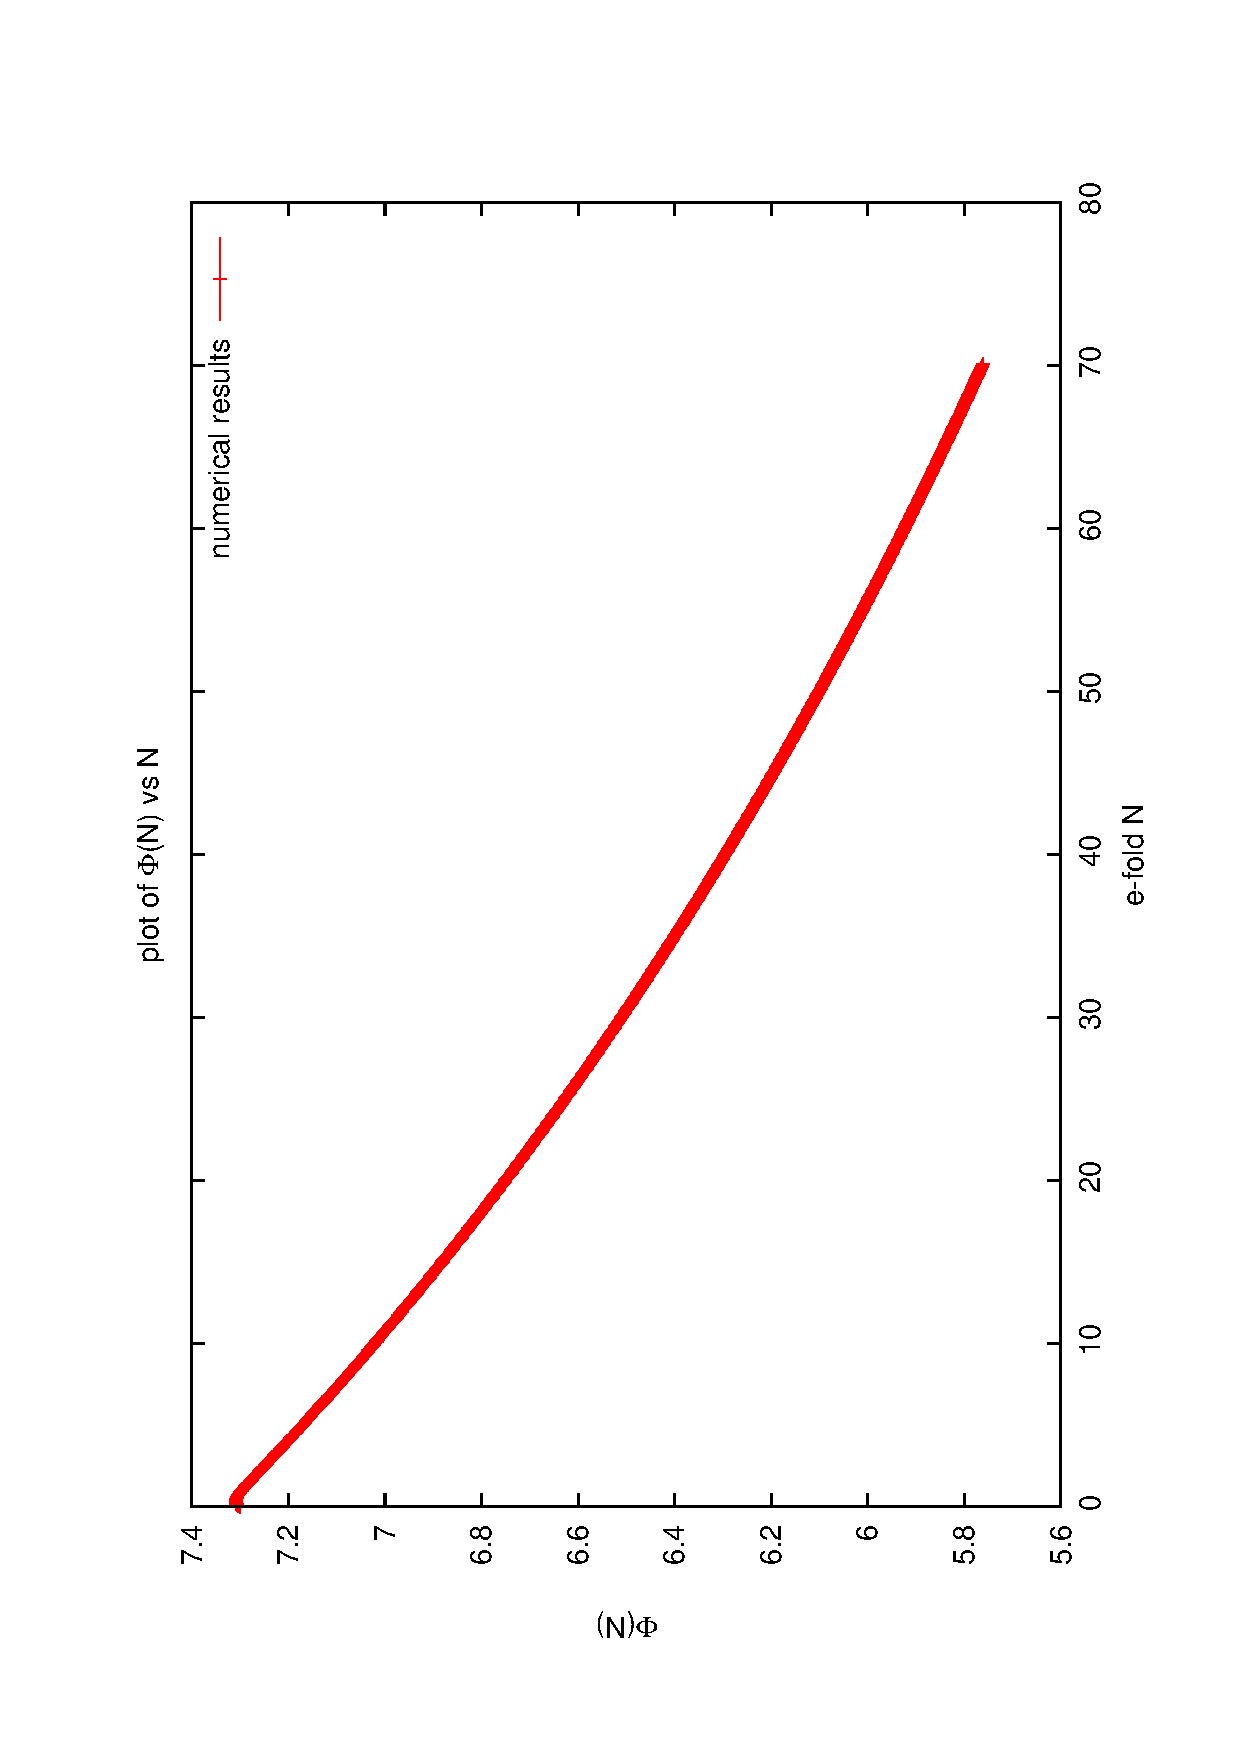
\includegraphics[scale=0.5]{phi_vs_N_small_field.png}
\caption[Plot of $\phi(N)$ vs $N$ during small field inflation]{Plot of $\phi(N)$ vs $N$ during small field inflation}
\end{center}
\end{figure}

\begin{figure}
\begin{center}
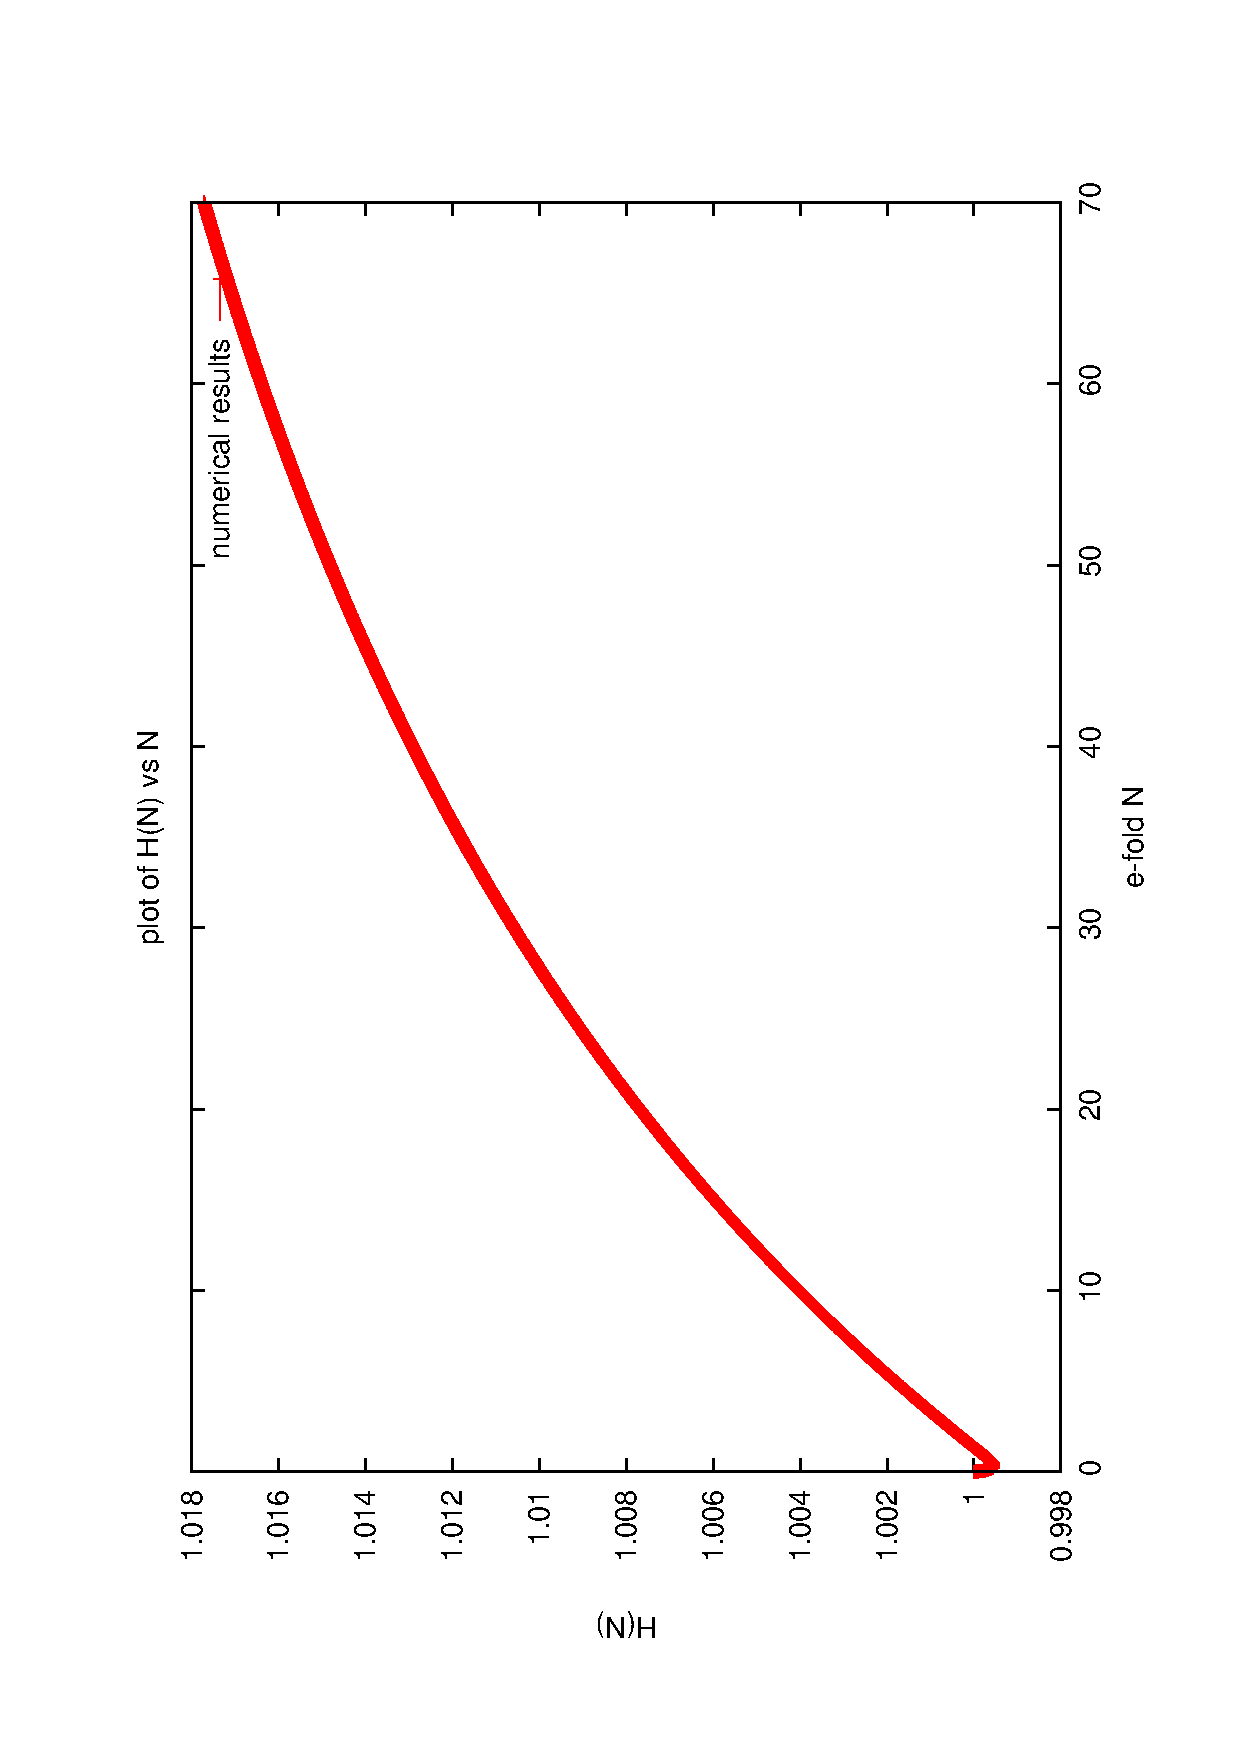
\includegraphics[scale=0.5]{H_vs_N_small_field.png}
\caption[Plot of $H(N)$ vs $N$ during small field inflation]{Plot of $H(N)$ vs $N$ during small field inflation}
\end{center}
\end{figure}

\begin{figure}
\begin{center}
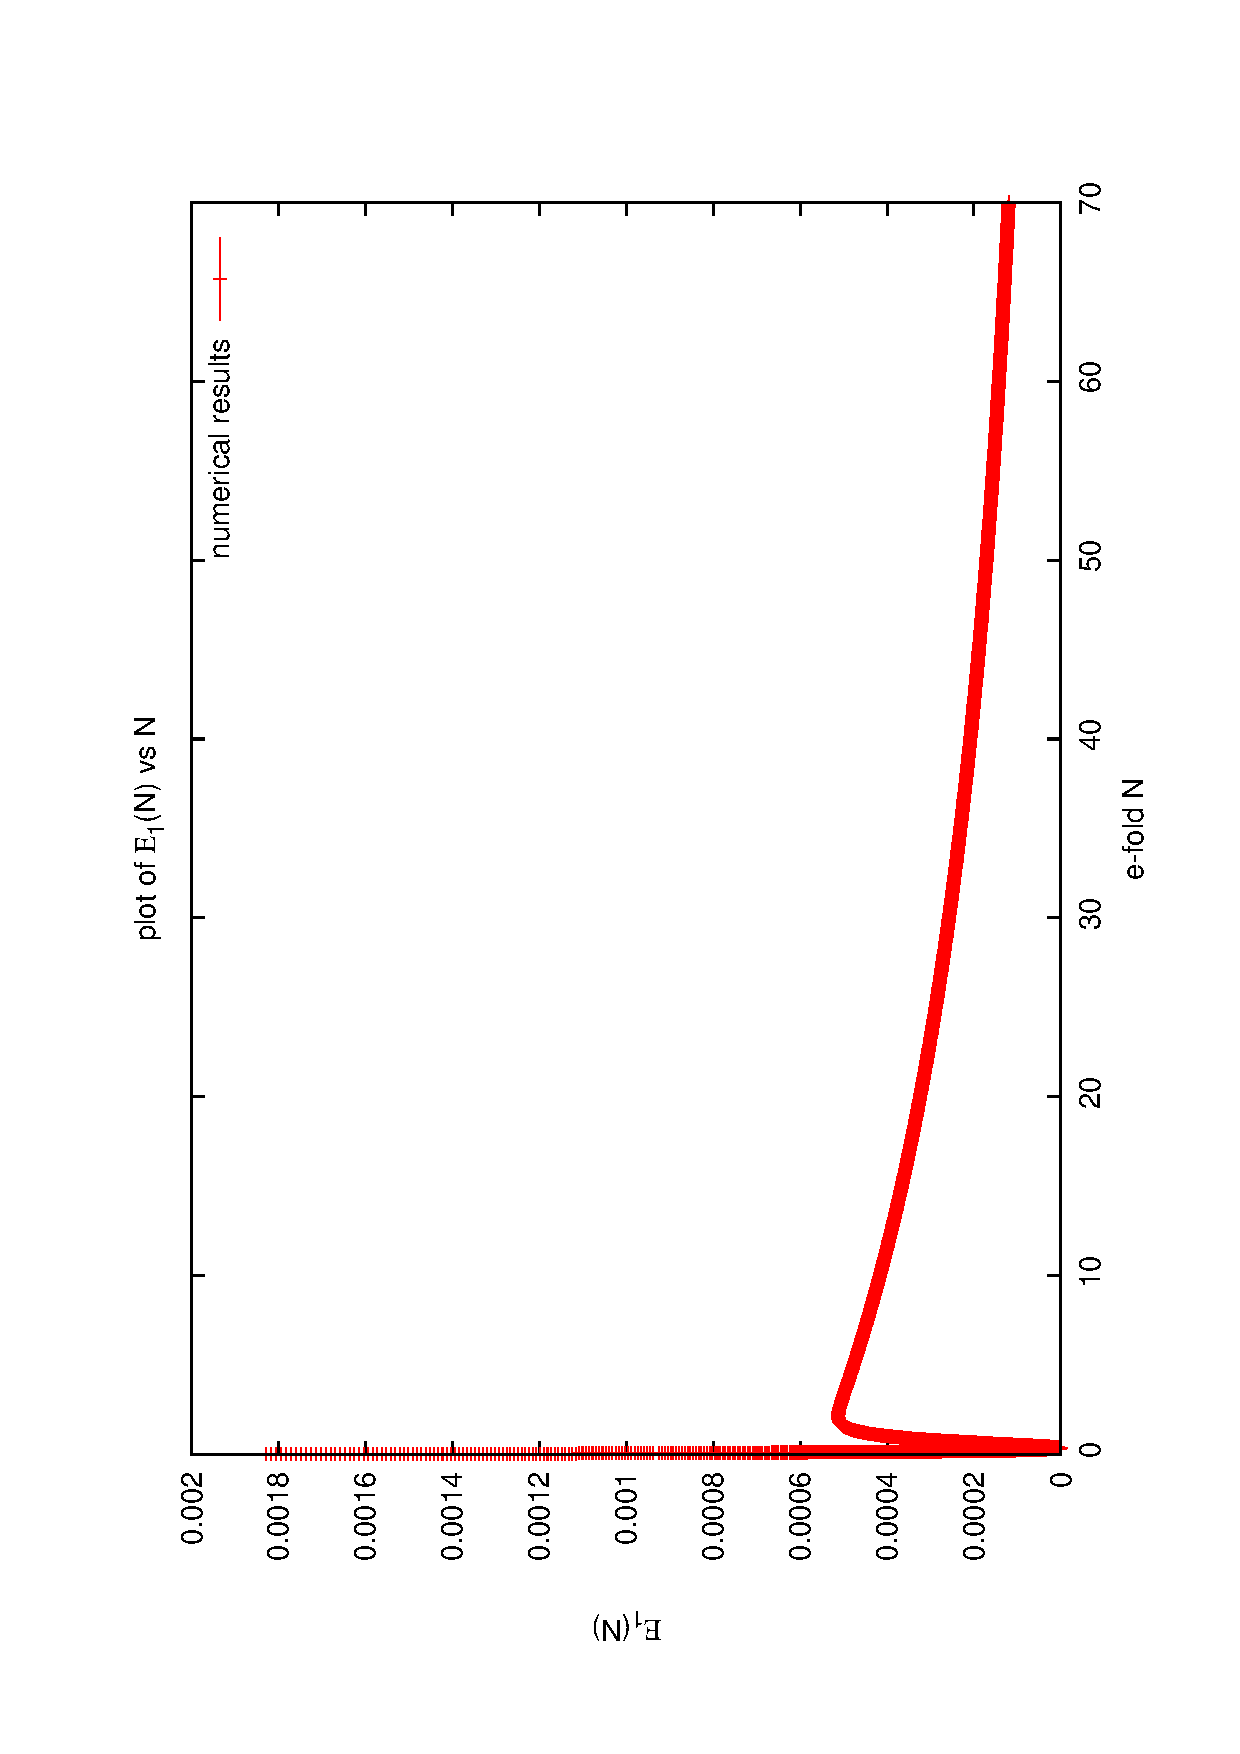
\includegraphics[scale=0.5]{eps1_vs_N_small_field.png}
\caption[Plot of $\epsilon 1(N)$ vs $N$ during small field inflation]{Plot of $\epsilon 1(N)$ vs $N$ during small field inflation}
\end{center}
\end{figure}

%\paragraph*{} just to test this ~\cite{Kodama:1985bj} %and ~\cite{Kazanas:1980tx}

%%%%%%%%%%%%%%%%%%%%%%%%%%%%%%%%%%%%%%%%%%%%%%%%%%%%%%%%%%%%%%%%%%%%%%%%%%%%%%%

\chapter{Summary}

%%%%%%%%%%%%%%%%%%%%%%%%%%%%%%%%%%%%%%%%%%%%%%%%%%%%%%%%%%%%%%%%%%%%%%%%%%%%%%%

%\nocite{Kodama:1985bj}
%\bibliographystyle{plain}
%\bibliography{tps}

%%%%%%%%%%%%%%%%%%%%%%%%%%%%%%%%%%%%%%%%%%%%%%%%%%%%%%%%%%%%%%%%%%%%%%%%%%%%%%%
\begin{thebibliography}{99}
%%%%%%%%%%%%%%%%%%%%%%%%%%%%%%%%%%%%%%%%%%%%%%%%%%%%%%%%%%%%%%%%%%%%%%%%%%%%%%%
%\bibitem{Sriramkumar L - 2009}
%L.~Sriramkumar, {\sl An introduction to inflation and cosmological perturbation theory}\/ (Current Science, 2009).

\bibitem{Linde}
Linde, A. D., Particle Physics and Inflationary Cosmology, Har-wood Academic, Switzerland, 1990.

\bibitem{B1}
Brandenberger, R. H., Rev. Mod. Phys., 1985, 57, 1.

\bibitem{B2}
Mukhanov, V. F., Feldman, H. A. and Brandenberger, R. H., Phys. Rep., 1992, 215, 203.

\bibitem{G1}
Giovannini, M., Int. J. Mod. Phys. D, 2005, 14, 363.

%%%%%%%%%%%%%%%%%%%%%%%%%%%%%%%%%%%%%%%%%%%%%%%%%%%%%%%%%%%%%%%%%%%%%%%%%%%%%%%
\end{thebibliography}
%%%%%%%%%%%%%%%%%%%%%%%%%%%%%%%%%%%%%%%%%%%%%%%%%%%%%%%%%%%%%%%%%%%%%%%%%%%%%%%

\begin{appendices}
\chapter{Python Code}
\begin{verbatim}

import numpy
import matplotlib.pyplot as plt
f = open('power_spectrum_power_law.dat','w')
q = 51.
V0 = (204./100.)*1e-08
t0 = (q*(3*q -1)/V0)**(1./2)
phi0 = 1.
dphi0 = (2.*q)**(1./2)/t0
Ni = 0.
Nf = 70. 
kp = 5.*1e-02
beta = -((2*q -1)/(q -1))
eps1a = ((beta +2)/(beta +1))
#V = lambda phi : V0*numpy.exp(-(2*q)**(1./2.)*(phi-phi_i))
V = lambda phi : V0*numpy.exp(-(2./q)**(1./2)*(phi -phi0))
dV = lambda phi : -(2./q)**(1./2)*V0*numpy.exp(-(2./q)**(1./2)*(phi -phi0))
H0 = ((1./3)*(dphi0**2/2. +V(phi0)))**(1./2.)
Dphi0 = dphi0/H0
def DDphi(N, phi0, Dphi0):
    return -(3 -Dphi0**2/2.)*Dphi0 -(dV(phi0)/(2*V(phi0)))*(6 -Dphi0**2)
def rk4_step(N, phi0, Dphi0, step):
    F1 = Dphi0
    f1 = DDphi(N, phi0, Dphi0)
    F2 = Dphi0 +f1*step/2.
    f2 = DDphi(N +step/2., phi0 +F1*step/2., Dphi0 +f1*step/2.)
    F3 = Dphi0 +f2*step/2.
    f3 = DDphi(N +step/2., phi0 +F2*step/2., Dphi0 +f2*step/2.)
    F4 = Dphi0 +f3*step
    f4 = DDphi(N +step, phi0 +F3*step, Dphi0 +f3*step)  
    return numpy.array([(f1 +2*f2 +2*f3 +f4)*step/6.]), numpy.array([(F1 +2*F2 +2*F3 +F4)*step/6.]) # [Dhk, hk] update
npts = 20000
step = (Nf-Ni)/(npts)
phi_array = numpy.array([phi0])
Dphi_array = numpy.array([Dphi0])
N_array = numpy.array([Ni]) 
N = Ni
while N < Nf:
    array = rk4_step(N, phi0, Dphi0, step)
    phi0 = phi0 + array[1]
    Dphi0 = Dphi0 + array[0]
    phi_array = numpy.append(phi_array,phi0)
    Dphi_array = numpy.append(Dphi_array,Dphi0)
    N += step
    N_array = numpy.append(N_array,N)
#plt.plot(numpy.linspace(0,70,npts+1), phi_array)
plt.cla()
plt.plot(N_array, phi_array)
plt.savefig('phi_vs_N.png')
eps0 = (3./2)*((dphi0**2)/(dphi0**2/2. + V(phi0)))
eps = 1./q 
#H = [((V(phi_array[i]))/(3 -Dphi_array[i]**2/2))**(1./2) for i in range(len(phi_array))]
phi = lambda N : phi_array[int((N-Ni)/step)]
Dphi = lambda N : Dphi_array[int((N-Ni)/step)]
H = lambda N : ((V(phi(N))/(3 -Dphi(N))**2/2))**(1./2)
DH = lambda N : H(N)*Dphi(N)
plt.cla()
plt.plot(N_array, numpy.asarray([str(H(i)).strip('[]') for i in N_array], dtype= numpy.float64)/H0)
plt.savefig('H_vs_N.png')
ai = 1e-05
eps1 = lambda N : Dphi_array[int((N-Ni)/step)]**2/2.
plt.cla()
plt.plot(N_array, [str(eps1(i)).strip('[]') for i in N_array])
plt.savefig('eps1_vs_N.png')
#z = [ai*numpy.exp(N_array[i])*Dphi_array[i] for i in range(len(N_array))]
z = lambda N: ai*numpy.exp(N)*Dphi(N)
A = lambda N : ai*numpy.exp(N)
def DDhk(k0, N, hk0, Dhk0):
    return -((3. +(DH(N)/H(N)))*Dhk0 +((k0/(A(N)*H(N)))**2)*hk0)
def rk4_step(k0, N, hk0, Dhk0, step):
    F1 = Dhk0
    f1 = DDhk(k0, N, hk0, Dhk0)
    F2 = Dhk0 +f1*step/2.
    f2 = DDhk(k0, N +step/2., hk0 +F1*step/2., Dhk0 +f1*step/2.)
    F3 = Dhk0 +f2*step/2.
    f3 = DDhk(k0, N +step/2., hk0 +F2*step/2., Dhk0 +f2*step/2.)
    F4 = Dhk0 +f3*step
    f4 = DDhk(k0, N +step, hk0 +F3*step, Dhk0 +f3*step)   
    return numpy.array([(f1 +2*f2 +2*f3 +f4)*step/6.], dtype=complex), numpy.array([(F1 +2*F2 +2*F3 +F4)*step/6.], dtype=complex) # [Dhk, hk] update
Nics_array = numpy.array([2.54198038578949765072641948787, 3.71629878321646094957559512976, 4.89061718064342424842477077165, 6.06493557807038754727394641354, 7.23925397549735084612312205543, 8.41357237292431414497229769732, 9.58789077035127744382147333808, 10.7622091677782407426704414080, 11.9365275652052040415198238617, 13.1108459626321673403690002649, 14.2851643600591306392181759068, 15.4594827574860939380673515487, 16.6338011549130572369165271905, 17.8081195523400205357657028324])
Nshs_array = numpy.array([18.9824379497669838346148777580, 20.1567563471939471334640541162, 21.3310747446209104323132297581, 22.5053931420478737311624054000, 23.6797115394748370300115810419, 24.8540299369018003288607566837, 26.0283483343287636277099323256, 27.2026667317557269265591079675, 28.3769851291826902254082834314, 29.5513035266096535242574592513, 30.7256219240366168231066348932, 31.8999403214635801219558105351, 33.0742587188905434208049861770, 34.2485771163175067196541618192])
Nics_arr = Ni + numpy.array((Nics_array-Ni)/step,dtype=int)*step
Nshss_arr = Ni + numpy.array((Nshs_array-Ni)/step,dtype=int)*step
k_min = 1e-6
k_max = 10
print 'lift off!'
k_vs_hk = numpy.zeros(1,dtype=complex)
i = 0
k0 = k_min
while k0 < k_max:
    print 'k0 = ', k0
    Nics = Nics_arr[i]
    Nshss = Nshss_arr[i]
    hk0 = numpy.zeros(1,dtype=complex)
    hk0.real = (((2.*k0)**(1./2))*A(Nics))**(-1.)
    Dhk0 = numpy.zeros(1,dtype=complex)
    Dhk0.real = -(1/A(Nics))*((2*k0)**(-1./2))
    Dhk0.imag = -((k0/2)**(1./2))/(A(Nics)*A(Nics)*H(Nics))
    print 'got Nics, hk0 and Dhk0'
    print 'starting from Nics'
    N = Nics
    while N < Nshss:
        #array = euler_step()
        array = rk4_step(k0, N, hk0, Dhk0, step)
        hk0 = hk0 + array[1]
        Dhk0 = Dhk0 + array[0]
        N += step
    k_vs_hk = numpy.append(k_vs_hk, hk0) 
    print N-step, Nshss, hk0, Dhk0, Nics
    print '\n'
    temp = 8*(k0)**3/(2*numpy.pi**2)*(numpy.absolute(hk0))**2
    f.write(str(k0)+"\t"+str(hk0.real)+"\t"+str(hk0.imag)+"\t"+str(temp)+"\n") 
    k0 = 10**(1./2)*k0
    i += 1
k_list = numpy.array([10**((-12 + i)/2.) for i in range(13)])
#print len(k_list), len(k_vs_hkhk)
TPS = [8*(k_list[i])**3/(2*numpy.pi**2)*(numpy.absolute(k_vs_hk[i+1]))**2 for i in range(len(k_list))]
print k_list, TPS
f.close()
plt.loglog(k_list, TPS)
plt.savefig('power_spectrum_power_law.png')

\end{verbatim}
\end{appendices}
%%%%%%%%%%%%%%%%%%%%%%%%%%%%%%%%%%%%%%%%%%%%%%%%%%%%%%%%%%%%%%%%%%%%%%%%%%%%%%%
\end{document}